% Appendix E: the timing of funding. Moved from the main text (former Section 7) on
% 2026-09-29 (revision plan 2, Package B), with three stated limits added. Terms: "the
% forward-looking funder's timing" (not "optimal timing"); ``gain from planning ahead''
% (not "timing gain").
\section{The timing of funding}\label{app:timing}

The funder holds a fixed budget for the whole horizon, and between rounds two things change: researchers produce research output, which the funder observes, and capabilities compound. In the main text the funder spends its budget in equal parts each round; this appendix asks whether it should spend early, evenly, or late, and how much the choice matters.

The strongest argument for spending early concerns fields whose researchers have few resources. A researcher without resources produces nothing, so the funder observes nothing and no capability grows; money held for later rounds therefore produces neither evidence nor growth in the meantime. On this argument a funder facing such a field should spend at once. The argument fails. A funder that spends everything in the first round allocates before observing any research output, and knows exactly as little as a funder that spends everything in the last round; in the extreme case of a field with no resources at all, the two produce identical expected research output. What the argument does establish is a complementarity: early spending enables observation and growth, and late spending exploits what early spending revealed. This complementarity favors putting some money early. It does not favor putting most of it early.\footnote{Among timings fixed in advance, the best timing that spends more than an even share in the early rounds loses to even spending by 1.6 percent of even spending's research output at negligible compounding and by 3.5 percent at the default compounding rate (six rounds, community with few resources).}

Our simulations bear this out: under complementarity, observation comes first and money second. Wherever capabilities compound at more than a negligible rate, the forward-looking funder spends less than an even share in the first round and spends the bulk once research output has revealed who is capable; spending late pays because money spent later is spent with more information, and because early research output compounds on its own (Figure~\ref{fig:timing-boundary}). Scarce baseline resources raise the early share and decreases the intensity of the effect, but does not reverse it.\footnote{Every parameter setting in which the forward-looking funder spends more than an even share early has a compounding rate $\epsilon \leq 0.03$, and there the center of mass of spending is within 0.005 of even.}

% Figure (S7): the schedule's tilt is governed by the compounding rate.
% y = budget-schedule center of mass (0.5 = even; above = late-leaning) of the
% forward funder; x = compounding rate eps (log scale); three baseline resource
% scales (r_min = 0.001 poor, 0.3, 3 rich). 200 seeds per cell.
% Data: fig8-boundary.dat, from sweep_results/resource_regime (hash 21b0d9a).
\begin{figure}[t]
\centering
\begin{tikzpicture}
\begin{axis}[
  width=0.82\textwidth, height=5.4cm,
  axis lines*=left,
  xmode=log,
  xmin=0.0001, xmax=0.85, ymin=0.48, ymax=0.68,
  xtick={0.0001, 0.01, 0.1, 0.85},
  xticklabels={0.0001, 0.01, 0.1, 0.85},
  ytick={0.5, 0.55, 0.6, 0.65},
  yticklabels={even, 0.55, 0.60, 0.65},
  xlabel={compounding rate $\epsilon$},
  ylabel={schedule center of mass},
  ylabel style={font=\small}, xlabel style={font=\small},
  tick label style={font=\small},
  axis line style={line width=0.4pt},
  tick style={line width=0.4pt, black},
  clip=false,
]
\addplot[gray, dashed, line width=0.4pt, domain=0.0001:0.85] {0.5};
\addplot[black, line width=0.7pt] table[x=eps, y=rich] {fig8-boundary.dat};
\addplot[black, line width=0.7pt] table[x=eps, y=mid]  {fig8-boundary.dat};
\addplot[black, line width=0.7pt] table[x=eps, y=poor] {fig8-boundary.dat};
\node[font=\small, anchor=west] at (axis cs:0.92,0.652) {resource-rich};
\node[font=\small, anchor=west] at (axis cs:0.92,0.566) {intermediate};
\node[font=\small, anchor=west] at (axis cs:0.92,0.521) {resource-poor};
\end{axis}
\end{tikzpicture}
\caption{The compounding rate, not resource poverty, sets how late the schedule leans. The schedule's center of mass (0.5 is even; higher is later) as the compounding rate $\epsilon$ increases, for three baseline resource scales. Settings: Appendix~\ref{app:simulation}.}
\label{fig:timing-boundary}
\end{figure}


How much a funder can learn from its own grants depends on their size. A researcher on a small grant produces research output nearly proportional to the grant and nearly independent of capability, so a funder whose grants are small learns almost nothing it can exploit later: in a field whose researchers have few resources, with no review signal, such a funder gains almost nothing over uniform funding. Large grants change this. As grants approach the scale of capability itself, research output separates the capable from the rest, and the funder recovers most of the value of discrimination, with timing that spends a small share early, so that research output can be observed, and the rest once the funder has learned who is capable (Figure~\ref{fig:depth-schedule}).\footnote{In a community whose researchers have few resources, with heavy-tailed capability and no review signal, over six rounds, the Bayesian funder's gain over uniform funding increases from a third of one percent of uniform funding's research output at the default grant size to nine percent at six times that size and ten percent at twelve times, roughly the gain a reliable review signal delivers at the default size.}

% Figure (S7): the optimal schedule at standard and deep funding.
% y = share of the budget spent in each round by the forward funder (S8); T = 6;
% poverty corner (r_min = 0.001), heavy tail (alpha_K = 1.3), no review signal
% (tau_K = 100), negligible compounding (eps = 1e-4), budget scaled against
% capability (budget_ref = "K"). b = 0.5: 50 seeds; b = 3: 24 seeds (max SE 0.006);
% round-1 share at b = 3 matches the canonical 200-seed run (0.104 vs 0.110).
% Data: fig7-schedule.dat, generated by for-claude/verify_s7.R (schedule addendum).
\begin{figure}[t]
\centering
\begin{tikzpicture}
\begin{axis}[
  width=0.82\textwidth, height=5.4cm,
  axis lines*=left,
  xmin=1, xmax=6, ymin=0.08, ymax=0.20,
  xtick={1, 2, 3, 4, 5, 6},
  ytick={0.10, 0.15, 0.167, 0.20},
  yticklabels={0.10, 0.15, even, 0.20},
  xlabel={round},
  ylabel={share of budget},
  ylabel style={font=\small}, xlabel style={font=\small},
  tick label style={font=\small},
  axis line style={line width=0.4pt},
  tick style={line width=0.4pt, black},
  clip=false,
]
\addplot[black, line width=0.7pt, mark=*, mark size=1.2pt] table[x=round, y=b05] {fig7-schedule.dat};
\addplot[black, line width=0.7pt, mark=o, mark size=1.4pt] table[x=round, y=b3] {fig7-schedule.dat};
\node[font=\small, anchor=west] at (axis cs:6.15,0.167) {standard depth ($b = 0.5$)};
\node[font=\small, anchor=west] at (axis cs:6.15,0.183) {deep grants ($b = 3$)};
\end{axis}
\end{tikzpicture}
\caption{Observation first, money after. The share of the budget the funder spends in
each of six rounds, in a resource-poor field with heavy-tailed capability and no
review signal. At standard depth (filled marks) the funder learns nothing from its
own thin grants and the optimal schedule is even. With deep grants (open marks) the
funder holds the first-round share below even and deploys the bulk once output has
revealed who is capable.}
\label{fig:depth-schedule}
\end{figure}


The shift of spending toward later rounds comes from the research output researchers produce whether or not they are funded: that research output compounds and reveals capability while the funder waits. Growth from grant-added research output alone would shift spending slightly toward earlier rounds, since earlier grants have longer to compound.\footnote{With growth from unfunded research output switched off, the center of mass of spending is 0.48 to 0.49, below even; with growth from grant-added research output switched off, 0.53 to 0.68 (five rounds).}

Finally, planning ahead is worth less than the signal provided by grant peer review, in every setting we test. Across all horizons and compounding rates in our sweeps, the forward-looking funder's gain over the myopic funder, which spends equal installments each round, stays below the review signal's value: at the default compounding rate and below it is smaller by an order of magnitude or more, and it approaches the signal's value only at the joint extreme of the highest compounding rate and the longest horizon we consider (Figure~\ref{fig:schedule-vs-signal}).\footnote{As a share of the research output that the forward-looking funder's funding adds, the gain from planning ahead ranges from indistinguishable from zero to 4.5 percent across the thirty tested parameter settings; the review signal's value in the same settings ranges from 7 to 27 percent.} The gain increases roughly with the square of the horizon over short horizons and levels off beyond five rounds. And it exists only where capability and resources are complements, as in our production function: under Cobb-Douglas production the gain from planning ahead is indistinguishable from zero and the forward-looking funder's timing stays within about a hundredth of even (Appendix~\ref{app:technology}, Table~\ref{tab:timing-technology}). For a funder thinking about how to maximize their impact, choosing whom to fund outweighs choosing when.

Three limits bound these results, and they are the reason the timing analysis sits in an appendix rather than the main text. First, the forward-looking funder is a certainty-equivalent planner (\S\ref{sec:model}): it treats future research output as equal to its expectation and does not value the information its own grants will generate, so it is not the Bayes-optimal sequential policy, and its gain is a lower bound on what planning ahead could be worth. Second, the gain combines two changes at once, when the money is spent and whom it reaches, because a funder that anticipates capability growth also values recipients differently; we do not separate the two, and ``gain from planning ahead'' names their sum. Third, the objective counts research output within the horizon only and assigns no value to the capability that remains at its end. A terminal value for capability would credit the capability that late grants build, which the horizon objective ignores, and also the compounded capability that early grants leave behind; we have not measured which effect is larger, so the size of the shift toward later rounds should be read as specific to the horizon objective.

% Figure (S7): what the schedule choice is worth, relative to the review signal.
% y = gain from deliberate scheduling (S8 - S5) as a share of the review signal's
% value (S8 - S7), by horizon T and compounding rate eps; negative gains floored at
% zero (all within noise of zero). Default parameters otherwise; 64-200 seeds per
% cell (T_run_smooth horizon_growth + horizon_long, hash 21b0d9a; re-derived
% in-session, verify_s7.R). Curves for eps in {0.05, 0.15, 0.3, 0.55, 0.85};
% eps = 0.05, 0.15, 0.55 were swept to T = 5 only.
\begin{figure}[t]
\centering
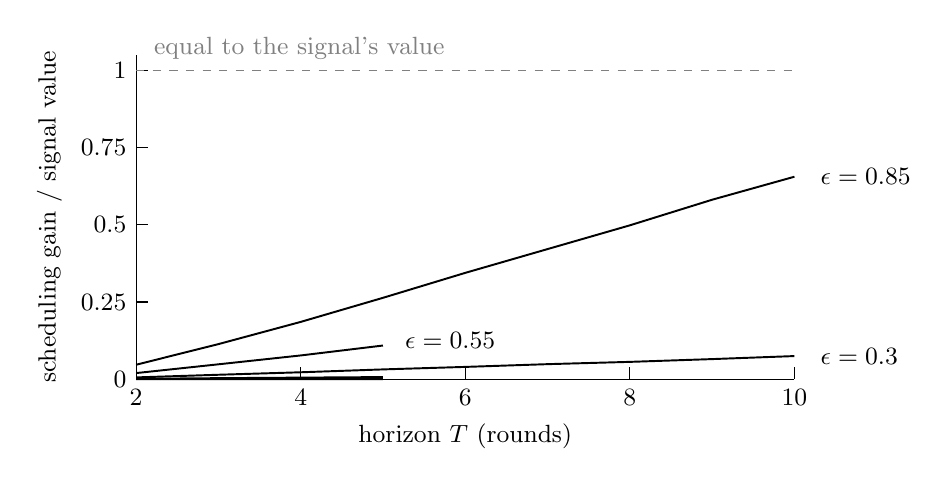
\begin{tikzpicture}
\begin{axis}[
  width=0.82\textwidth, height=5.7cm,
  axis lines*=left,
  xmin=2, xmax=10, ymin=0, ymax=1.05,
  xtick={2, 4, 6, 8, 10},
  ytick={0, 0.25, 0.5, 0.75, 1},
  yticklabels={0, 0.25, 0.5, 0.75, 1},
  xlabel={horizon $T$ (rounds)},
  ylabel={scheduling gain / signal value},
  ylabel style={font=\small}, xlabel style={font=\small},
  tick label style={font=\small},
  axis line style={line width=0.4pt},
  tick style={line width=0.4pt, black},
  clip=false,
]
\addplot[gray, dashed, line width=0.4pt, domain=2:10] {1};
\node[font=\small, gray, anchor=south west] at (axis cs:2.1,1.005) {equal to the signal's value};
\addplot[black, line width=0.7pt] coordinates {(2,0.0468) (3,0.1136) (4,0.1855) (5,0.2635) (6,0.3443) (7,0.4213) (8,0.4982) (9,0.5811) (10,0.6556)};
\addplot[black, line width=0.7pt] coordinates {(2,0.0198) (3,0.0482) (4,0.0769) (5,0.1090)};
\addplot[black, line width=0.7pt] coordinates {(2,0.0058) (3,0.0144) (4,0.0224) (5,0.0317) (6,0.0398) (7,0.0487) (8,0.0561) (9,0.0651) (10,0.0749)};
\addplot[black, line width=0.7pt] coordinates {(2,0.0012) (3,0.0034) (4,0.0051) (5,0.0069)};
\addplot[black, line width=0.7pt] coordinates {(2,0.0000) (3,0.0002) (4,0.0001) (5,0.0000)};
\node[font=\small, anchor=west] at (axis cs:10.2,0.656) {$\epsilon = 0.85$};
\node[font=\small, anchor=west] at (axis cs:5.15,0.126) {$\epsilon = 0.55$};
\node[font=\small, anchor=west] at (axis cs:10.2,0.075) {$\epsilon = 0.3$};
\end{axis}
\end{tikzpicture}
\caption{Choosing whom outweighs choosing when. The gain from deliberate scheduling
(a funder that plans its budget's spread over the horizon, over one that spends even
installments and re-decides each round) as a share of the review signal's value, by
horizon and compounding rate $\epsilon$; the default rate is $0.3$. In every setting
we test the gain is below the signal's value: an order of magnitude below or more at
the default rate and below, and approaching the signal's value only at the joint
extreme of the highest rate and the longest horizon. The two lowest curves, at $\epsilon = 0.15$ and $0.05$, and the curve at $0.55$ were
swept to five rounds.}
\label{fig:schedule-vs-signal}
\end{figure}

